\documentclass{beamer}
\usepackage{ctex, hyperref}
\usepackage[T1]{fontenc}

% other packages
\usepackage{latexsym,amsmath,xcolor,multicol,booktabs,calligra}
\usepackage{graphicx,pstricks,listings,stackengine}
\usepackage[normalem]{ulem}

\author{userElaina}
\title{Chains: LLM + Crowdsource}
\institute{School of AI}
\date{2024.06.27}
\usepackage{JilinUniv}

\def\cmd#1{\texttt{\color{red}\footnotesize $\backslash$#1}}
\def\env#1{\texttt{\color{blue}\footnotesize #1}}
\definecolor{deepblue}{rgb}{0,0,0.5}
\definecolor{deepred}{rgb}{0.6,0,0}
\definecolor{deepgreen}{rgb}{0,0.5,0}
\definecolor{halfgray}{gray}{0.55}

\lstset{
    basicstyle=\ttfamily\small,
    keywordstyle=\bfseries\color{deepblue},
    emphstyle=\ttfamily\color{deepred},    % Custom highlighting style
    stringstyle=\color{deepgreen},
    numbers=left,
    numberstyle=\small\color{halfgray},
    rulesepcolor=\color{red!20!green!20!blue!20},
    frame=shadowbox,
}

\begin{document}

\kaishu
\begin{frame}
    \titlepage
    \begin{figure}[htpb]
        \begin{center}
            
\includegraphics[width=0.15\linewidth]{pic/Jilin_University_Logo.eps}
        \end{center}
    \end{figure}
\end{frame}

% \begin{frame}
% \tableofcontents[sectionstyle=show,subsectionstyle=show/shaded/hide,subsubsectionstyle=show/shaded/hide]
% \end{frame}

\section{CoT}

\begin{frame}{Baseline}
    \begin{figure}[c]
        \centering
        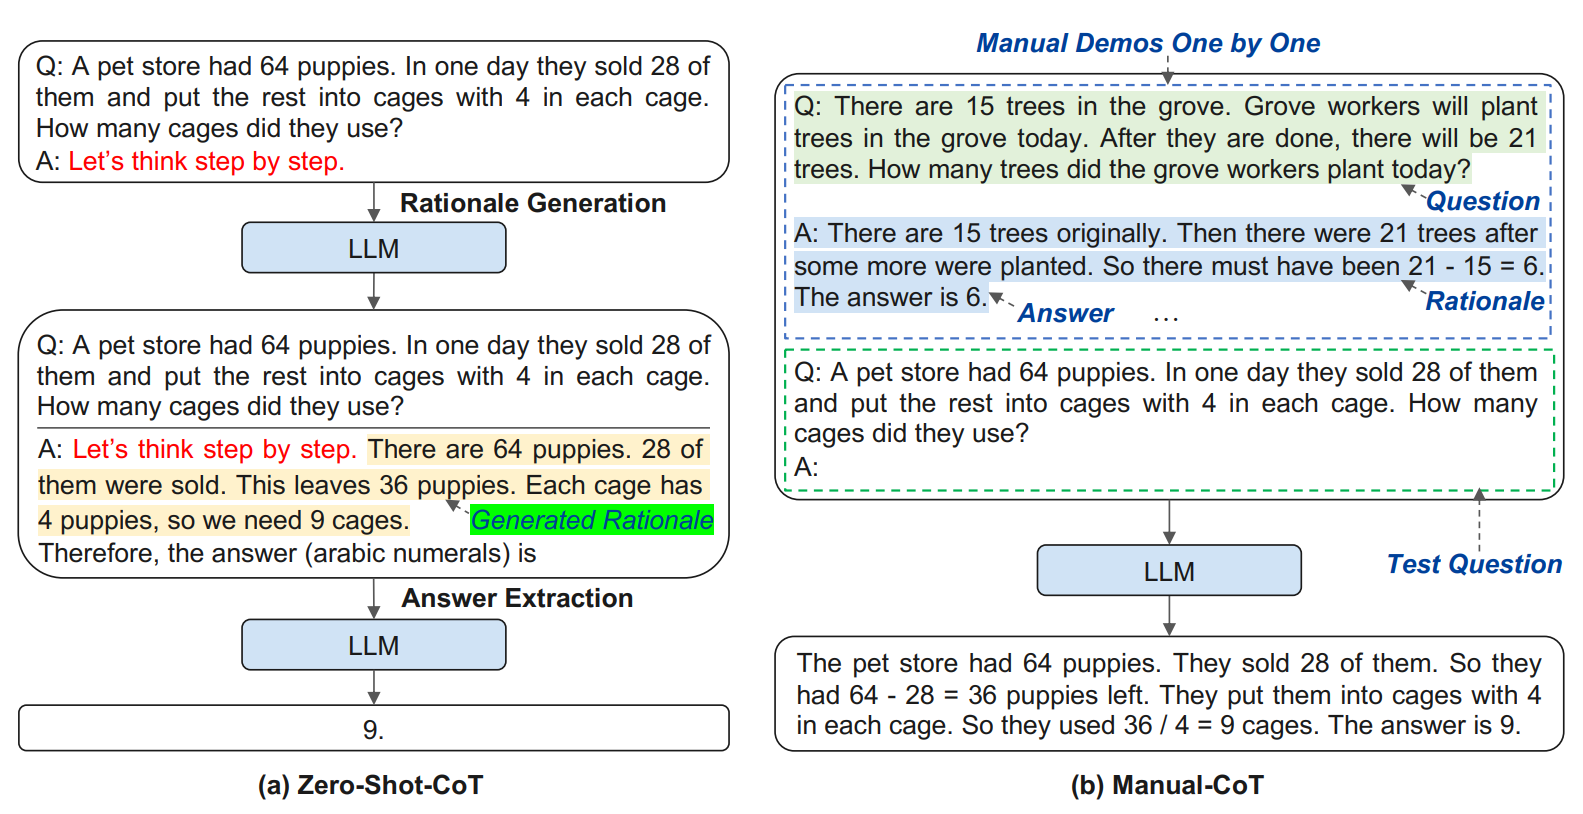
\includegraphics[height=.7\textheight]{pic/6.png}
        \caption{Zero-Shot-CoT \& Manual-CoT}
    \end{figure}
\end{frame}

\begin{frame}{AutoCoT}
    \begin{figure}[c]
        \centering
        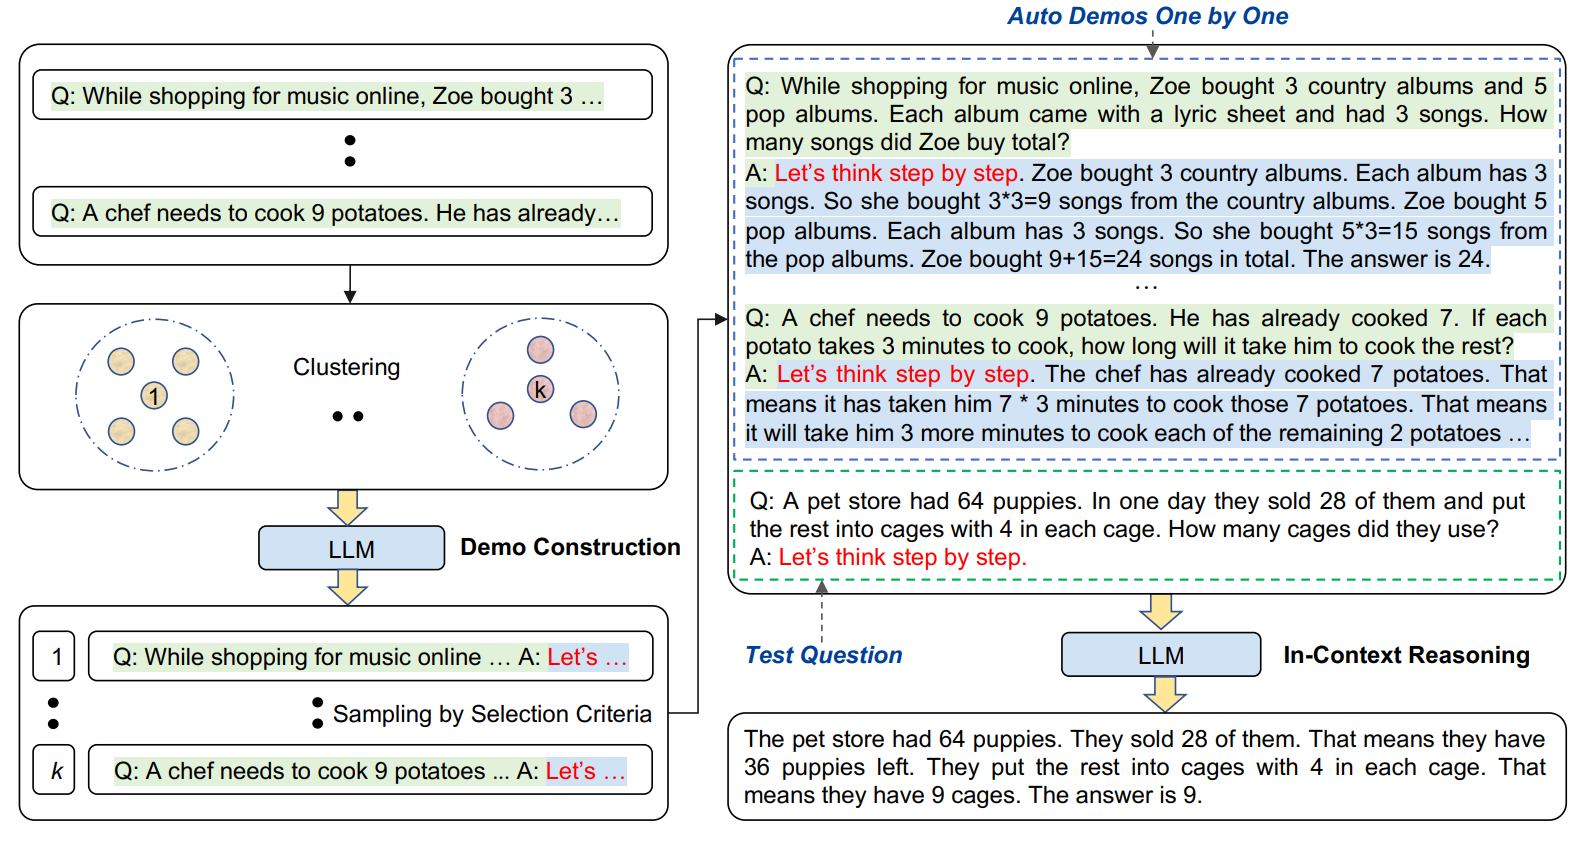
\includegraphics[height=.7\textheight]{pic/7.png}
        \caption{Automatic Chain of Thought Prompting in Large Language Models}
    \end{figure}
\end{frame}

\section{LangChain}

\begin{frame}{LangChain}
    \begin{itemize}
        \item Framework
        \item Prompt, AI Chains, \textbf{API}, ...
    \end{itemize}
\end{frame}

\section{AI Chains}

\begin{frame}{AI Chains}
    AI Chains: Transparent and Controllable Human-AI Interaction by Chaining Large Language Model Prompts
    \begin{itemize}
        \item Human-AI Interaction
        \item "Chain"
    \end{itemize}
\end{frame}

\begin{frame}{Response Biases}
    \begin{figure}[c]
        \centering
        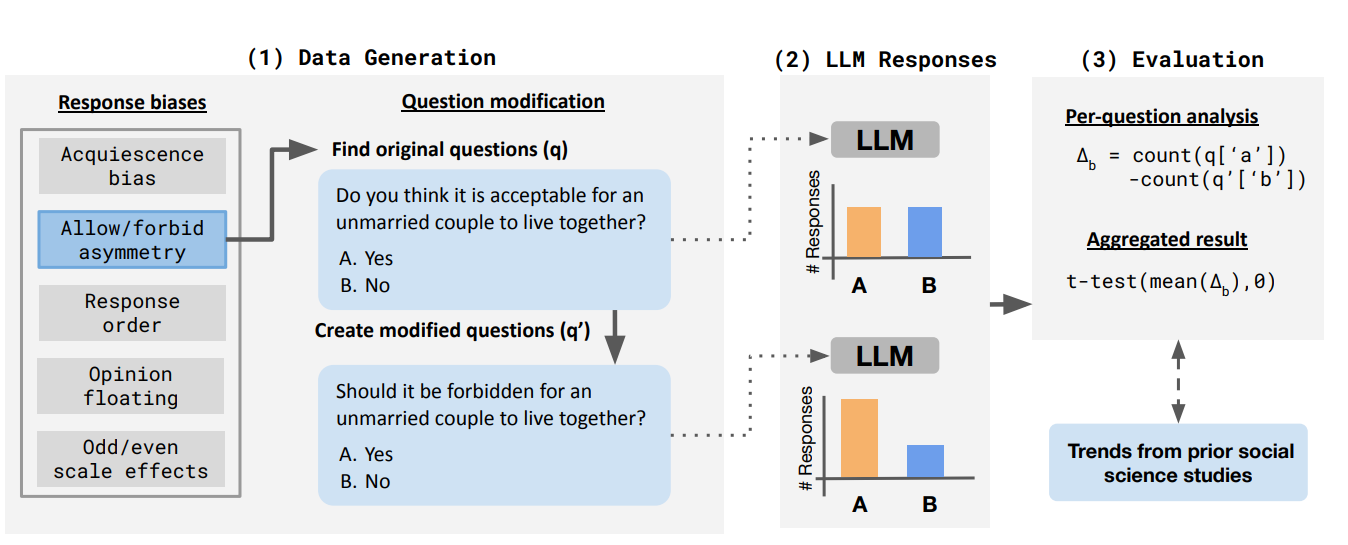
\includegraphics[height=.5\textheight]{pic/5.png}
        \caption{Do LLMs exhibit human-like response biases? A case study in survey design}
    \end{figure}
\end{frame}

\begin{frame}{Response Biases}
    Do LLMs exhibit human-like response biases? A case study in survey design
    \begin{itemize}
        \item Sensitivity: Diff
    \end{itemize}
\end{frame}

\section{LLM Chains}

\begin{frame}{LLM Chains}
    Designing LLM Chains by Adapting Techniques from Crowdsourcing Workflows
    \begin{itemize}
        \item Design
        \item 2023.08
        \item Workers:
        \begin{itemize}
            \item crowdworkers
            \item LLMs
            \item user
        \end{itemize}
    \end{itemize}
\end{frame}

\begin{frame}{Cascade}
    \begin{figure}[c]
        \centering
        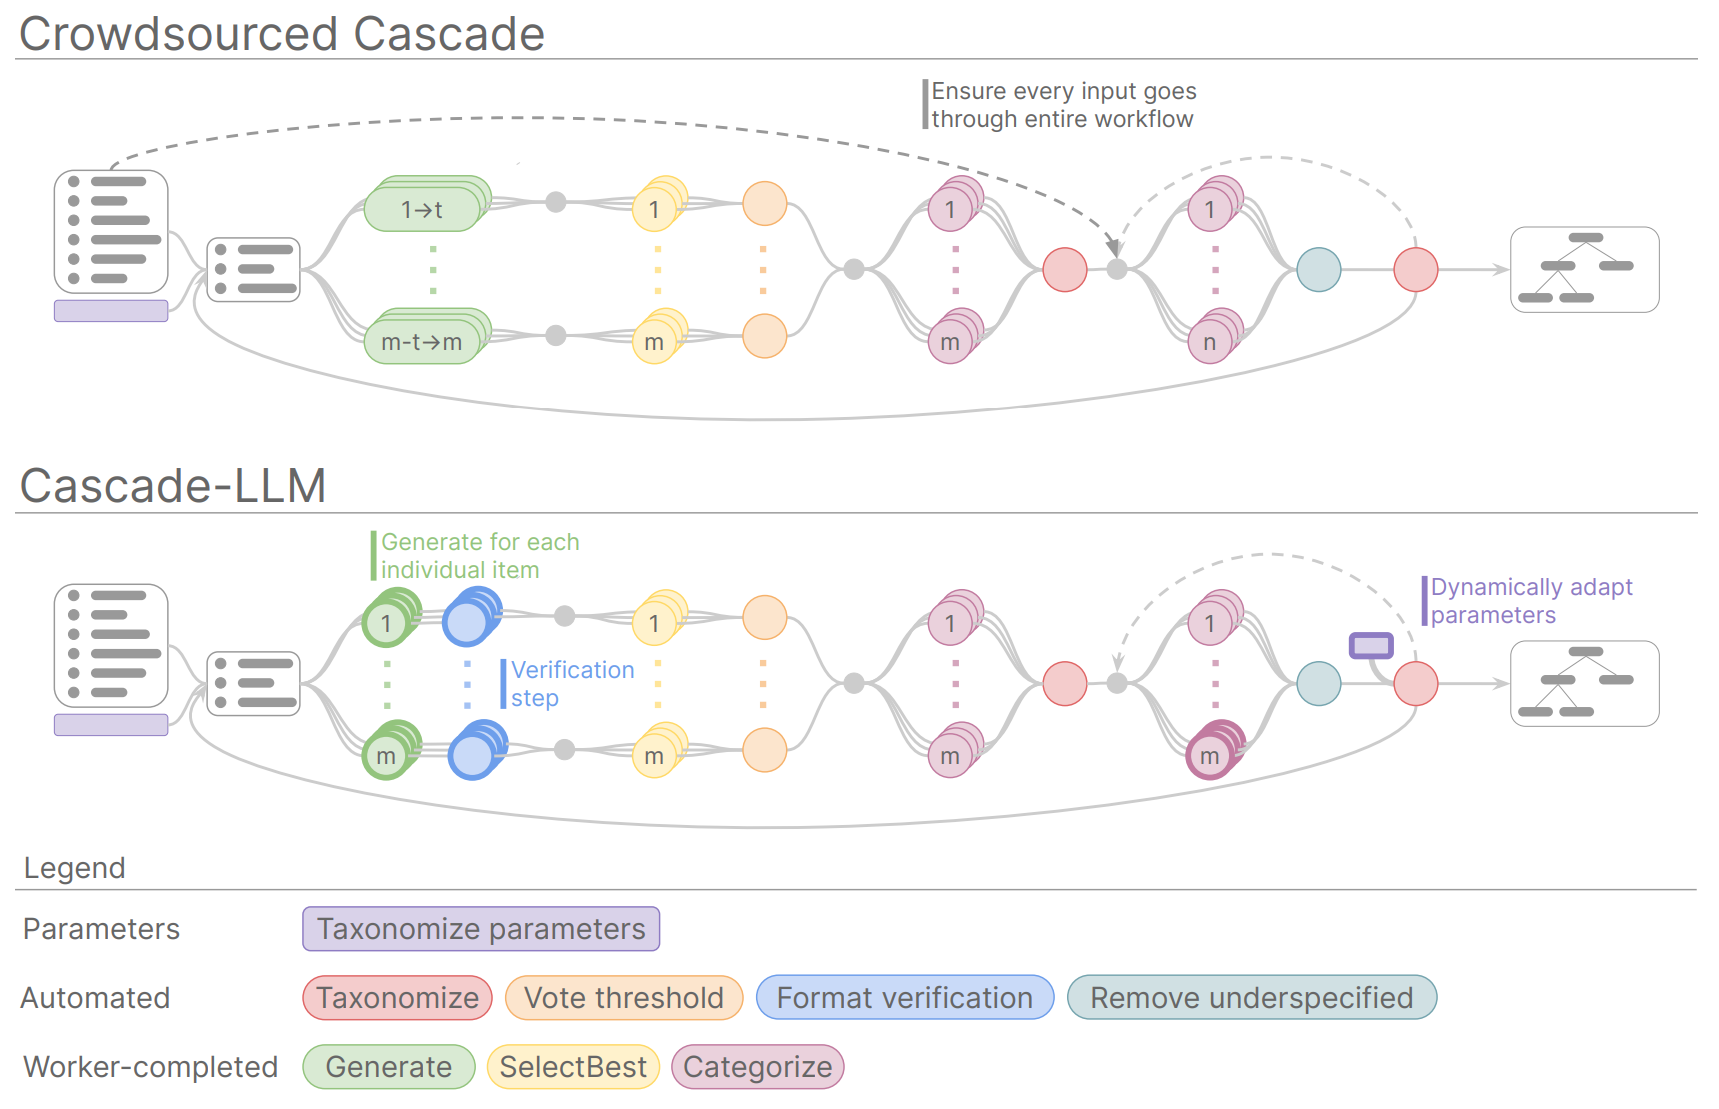
\includegraphics[height=.8\textheight]{pic/2.png}
        \caption{Cascade: Crowdsourcing Taxonomy Creation}
    \end{figure}
\end{frame}

\begin{frame}{Soylent}
    \begin{figure}[c]
        \centering
        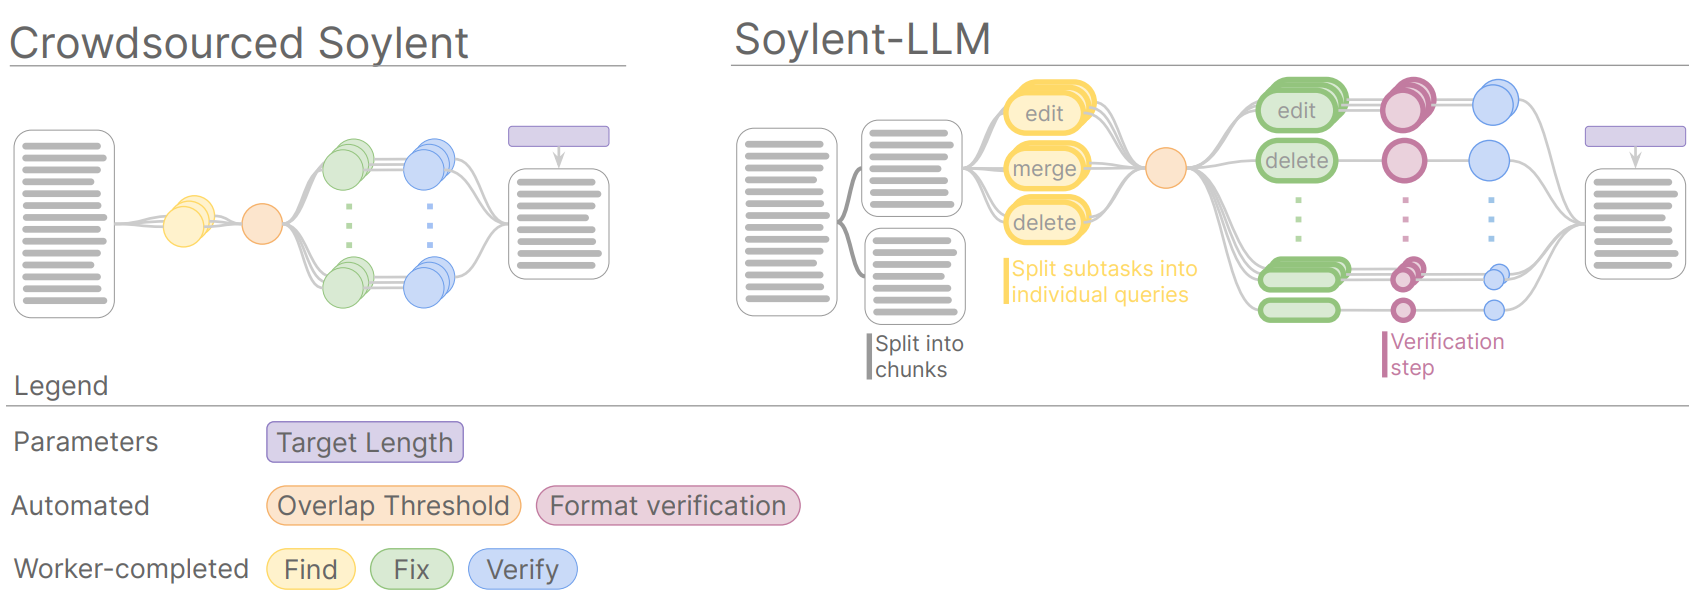
\includegraphics[height=.5\textheight]{pic/3.png}
        \caption{Soylent: A Word Processor with a Crowd Inside}
    \end{figure}
\end{frame}

\begin{frame}{Mechanical Novel}
    \begin{figure}[c]
        \centering
        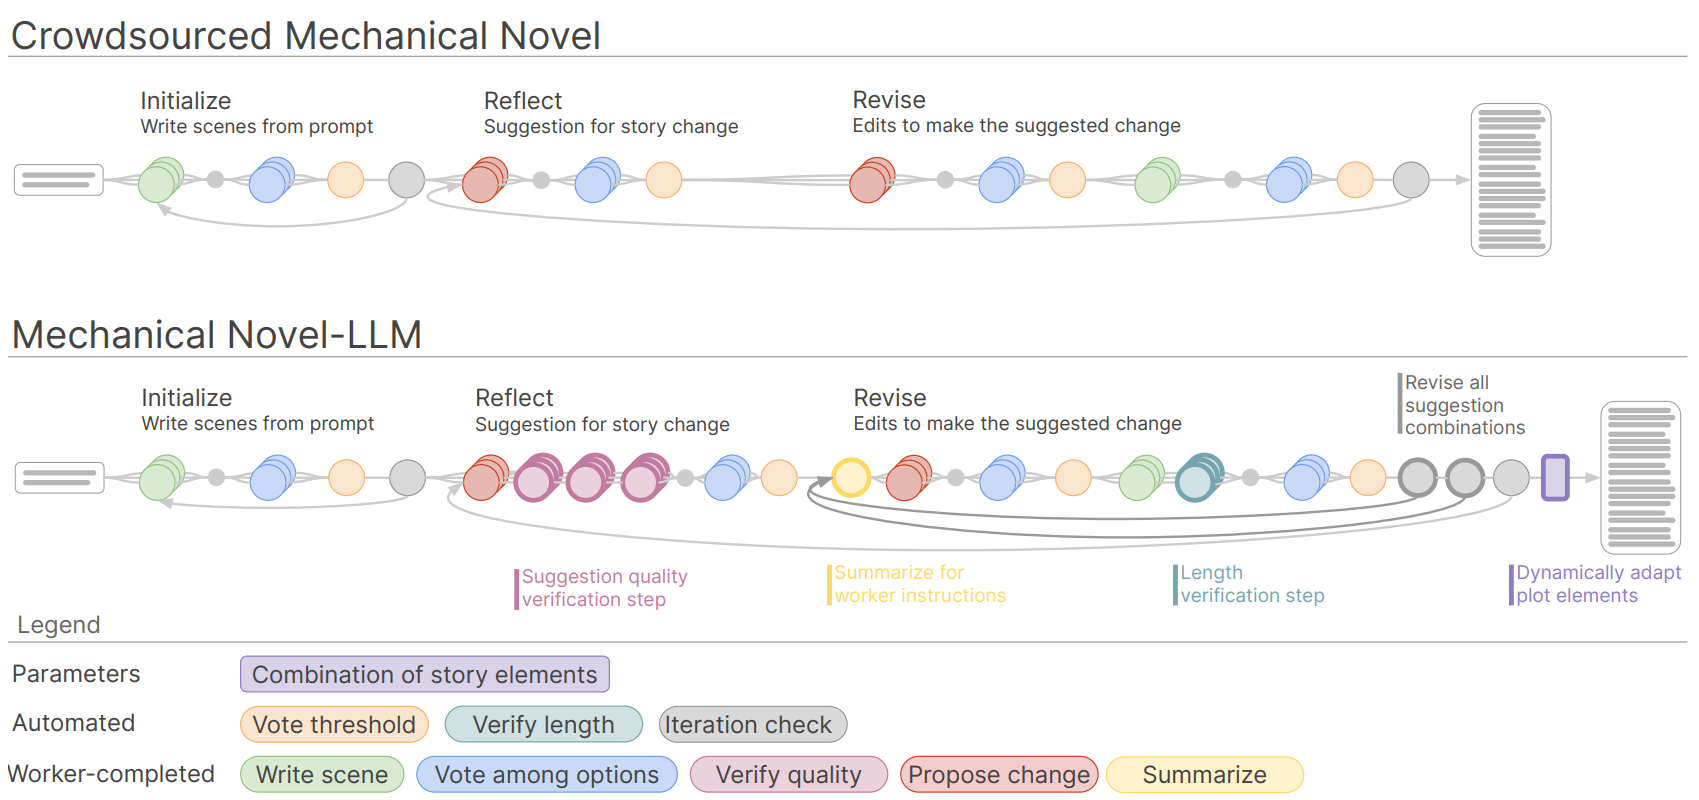
\includegraphics[height=.6\textheight]{pic/4.png}
        \caption{Mechanical Novel: Crowdsourcing Complex Work through Reflection and Revision}
    \end{figure}
\end{frame}

\begin{frame}{Prompt + Crowdsource}
    Revisiting Prompt Engineering via Declarative Crowdsourcing
    \begin{itemize}
        \item The 1st work
        \item "Declarative Crowdsourcing"
        \item Sorting:
        \begin{itemize}
            \item Sorting
            \item Pairwise
            \item Rating
            \item Hybrid Coarse -> Fine-grained Prompting
        \end{itemize}
    \end{itemize}
\end{frame}

\section{Idea}

\begin{frame}{Idea 1}
    \begin{itemize}
        \item Baseline: AI Chains
        \item AI Graph
    \end{itemize}
\end{frame}

\begin{frame}{Idea 2}
    \begin{itemize}
        \item Baseline: Designing LLM Chains(?)
        \item LLM Chains (Workflows) for Creative Tasks
        \item Dynamic and Communicative Architectures
    \end{itemize}
\end{frame}

\begin{frame}{Idea 3}
    \begin{itemize}
        \item Baseline: Cascade (or Other Algo) + Crowdworks(?)
        \item LLMs as Workers
        \item Cost?
        \item Creative Tasks?
    \end{itemize}
\end{frame}

\begin{frame}{Idea 4}
    \begin{itemize}
        \item LangChain
        \item Baseline: Designing LLM Chains
        \item API as Workers
        \item (LLM + Crowdworkers + User) + API
    \end{itemize}
\end{frame}

\end{document}

% Q model para
